\documentclass[twoside,a4paper]{article}
\usepackage{geometry}
\usepackage{ctex, hyperref}
\geometry{margin=1.5cm, vmargin={0pt,1cm}}
\setlength{\topmargin}{-1cm}
\setlength{\paperheight}{29.7cm}
\setlength{\textheight}{25.3cm}

% useful packages.
\usepackage{graphicx}
\usepackage{subcaption}
\usepackage{amsfonts}
\usepackage{amsmath}
\usepackage{amssymb}
\usepackage{amsthm}
\usepackage{enumerate}
\usepackage{graphicx}
\usepackage{multicol}
\usepackage{fancyhdr}
\usepackage{layout}
\usepackage{listings}%插入代码
\usepackage{ctex}%引入中文包
\usepackage{graphicx}%插入图片的包
\usepackage{geometry}%设置A4纸页边距的包
\usepackage{url}
\usepackage{stfloats}
\usepackage{float}
\usepackage{amssymb}
\usepackage{listings}
\usepackage{tikz}
% some common command
\newcommand{\dif}{\mathrm{d}}
\newcommand{\avg}[1]{\left\langle #1 \right\rangle}
\newcommand{\difFrac}[2]{\frac{\dif #1}{\dif #2}}
\newcommand{\pdfFrac}[2]{\frac{\partial #1}{\partial #2}}
\newcommand{\OFL}{\mathrm{OFL}}
\newcommand{\UFL}{\mathrm{UFL}}
\newcommand{\fl}{\mathrm{fl}}
\newcommand{\op}{\odot}
\newcommand{\Eabs}{E_{\mathrm{abs}}}
\newcommand{\Erel}{E_{\mathrm{rel}}}

\begin{document}

\pagestyle{fancy}
\fancyhead{}
\lhead{褚朱钇恒 (3200104144)}
\chead{Numerical PDE homework \#5}
\rhead{2023.6.11}

\section{Exercise 12.11}
根据定义12.10,我们有:

$$U_i^{n+1}-(rU_{i-1}^{n+1} - 2rU_i^{n+1} + rU_{i+1}^{n+1}) = rU_{i-1}^n + 2(1-r)U_i^n + rU_{i+1}^n, \quad (i = 1,2,\cdots,m)$$

当 $i=1$ 时,我们有:

$$(1+r)U^{n+1}_1 - \frac{r}{2}U^{n+1}_2 = (1-r)U^n_1+\frac{r}{2}U^n_2+\frac{r}{2}(U_0^n+U^{n+1}0) = (1-r)U^n_1+\frac{r}{2}U^n_2+\frac{r}{2}(g_0(t_n)+g_0(t{n+1}))$$

类似地,当 $i=m+1$ 时也成立。

令 $U^n = (U_1^n, U_2^n,\cdots, U_m^n)'$,$r=\frac{k\nu}{h^2}$,则有:

$$(I - \frac{k}{2}A)U^{n+1} = (I+\frac{k}{2}A)U^n+b^n,$$

其中,

$$A = \frac{\nu}{h^2}\begin{pmatrix}
-2 & 1 & & & & \\
1 & -2 & 1 & & & \\
& 1 & -2 & 1 & & \\
& & \ddots & \ddots & \ddots & \\
& & & 1 & -2 & 1\\
& & & & 1 & -2
\end{pmatrix}, 
\quad 
b^n = \frac{r}{2} \begin{pmatrix}
g_0(t_n)+g_0(t_{n+1})\\
0\\
\vdots\\
0\\
g_1(t_n)+ g_1(t_{n+1})
\end{pmatrix}$$

\section{Exercise 12.26}
我们可以利用一步法的稳定函数来推导 $\theta$ 方法的稳定性条件。对于线性常系数偏微分方程 $u_t = \nu u_{xx}$,用 $\theta$ 方法进行离散化,得到如下迭代公式:
$$
u_i^{n+1} = \frac{\theta k\nu}{h^2}(u_{i+1}^n - 2u_i^n + u_{i-1}^n) + (1-\theta)u_i^n.
$$
我们对其进行变量替换,定义 $w^n = (w_1^n,w_2^n,\dots,w_N^n)^T$,其中 $w_i^n = u_i^n$,并将 $\theta k\nu/h^2$ 记为 $\lambda$,则上式可以表示为 $w^{n+1} = A_\theta w^n$,其中
$$
A_\theta = \begin{pmatrix}
1-2\lambda\theta & \lambda\theta & & \\
\lambda\theta & 1-2\lambda\theta & \lambda\theta & \\
& \ddots & \ddots & \ddots \\
& & \lambda\theta & 1-2\lambda\theta \\
\end{pmatrix}.
$$
我们可以证明,当 $\theta\in[1/2,1]$ 时,矩阵 $A_\theta$ 的所有特征值均具有非负实部,因此方法是无条件稳定的。当 $\theta\in[0,1/2)$ 时,矩阵 $A_\theta$ 的特征多项式为
$$
p(\lambda) = (-1)^N\lambda^N + (2\lambda-1+\theta h^2\nu^{-1})\lambda^{N-1} - \lambda^{N-2}\theta h^2\nu^{-1}(1-2\theta)(N-1),
$$
其中 $N$ 是空间离散化的网格数。根据谱半径的定义,$A_\theta$ 的特征值的模长的上界为 $|\lambda_{\max}| \leq \rho(A_\theta)$,其中 $\rho(A_\theta)$ 是 $A_\theta$ 的谱半径。因此要使方法稳定,必须满足 $\rho(A_\theta)\leq 1$。令 $p(\lambda) = 0$,则有
$$
\lambda = \frac{1}{2}\left(1-\theta h^2\nu^{-1}\pm\sqrt{(1-\theta h^2\nu^{-1})^2 - 4\theta(1-2\theta)(N-1)h^2\nu^{-1}}\right).
$$
注意到 $\theta(1-2\theta)\leq 1/4$,因此根据根的公式,有 $\sqrt{(1-\theta h^2\nu^{-1})^2 - 4\theta(1-2\theta)(N-1)h^2\nu^{-1}} \leq |1-\theta h^2\nu^{-1}|$。因此我们可以得到 $\lambda$ 的模长的上界为
$$
|\lambda| \leq \frac{1}{2}\left[|1-\theta h^2\nu^{-1}| + \sqrt{(1-\theta h^2\nu^{-1})^2 - 4\theta(1-2\theta)(N-1)h^2\nu^{-1}}\right].
$$
为了保证方法稳定,需要使 $|\lambda| \leq 1$,即
$$
|1-\theta h^2\nu^{-1}| + \sqrt{(1-\theta h^2\nu^{-1})^2 - 4\theta(1-2\theta)(N-1)h^2\nu^{-1}} \leq 2.
$$
由于 $\sqrt{(1-\theta h^2\nu^{-1})^2 - 4\theta(1-2\theta)(N-1)h^2\nu^{-1}}$ 是非负实数,因此上式等价于
$$
1-\theta h^2\nu^{-1} + \sqrt{(1-\theta h^2\nu^{-1})^2 - 4\theta(1-2\theta)(N-1)h^2\nu^{-1}} \leq 2.
$$
将 $\sqrt{(1-\theta h^2\nu^{-1})^2 - 4\theta(1-2\theta)(N-1)h^2\nu^{-1}}$ 移到不等式右边,平方两边,可得
$$
(1-\theta h^2\nu^{-1})^2 - 4\theta(1-2\theta)(N-1)h^2\nu^{-1} \leq (3-\theta h^2\nu^{-1})^2.
$$
将 $\theta$ 方法的时间步长 $k$ 替换为 $\nu k/h^2$,可得
$$
k \leq \frac{h^2}{2(1-2\theta)\nu}.
$$
因此,当 $\theta\in[0,1/2)$ 时,为保证 $\theta$ 方法的稳定性,时间步长 $k$ 必须满足 $k\leq h^2/2(1-2\theta)\nu$。综上所述,引理得证。
\section{Exercise 12.41}
因为对于任何 $U\in L^1(h_{\mathbb{Z}})\cap L^2(h_{\mathbb{Z}})$,我们有
$$
\frac{1}{\sqrt{2\pi}}\int_{-\pi/h}^{\pi/h}e^{imh\xi}\left(\frac{1}{\sqrt{2\pi}}\sum_{n\in \mathbb{Z}}e^{inh\xi}U_{nh}\right)d\xi=\frac{1}{2\pi}\sum_{n\in \mathbb{Z}}\int_{-\pi}^\pi e^{-i(n-m)t}U_ndt
$$
$$
=\frac{1}{2\pi}\int_{-\pi}^\pi U_m dt= U_m
$$
其中 $t = h\xi$,当 $n \neq m$ 时,$\int_{-\pi}^\pi e^{-i(n - m)t}U_ndt = 0$。因此,对于任何 $U\in L^1(h_{\mathbb{Z}})\cap L^2(h_{\mathbb{Z}})$ 中的网格函数,我们可以通过傅里叶变换和逆傅里叶变换来恢复它。
\section{Exercise 12.48}
我们考虑对于方程 $\frac{\partial u}{\partial t}= \nu \frac{\partial^2 u}{\partial x^2}$,使用 $\theta$ 方法进行离散化。具体而言,我们将时间和空间分别离散化为 $t_n=nk$ 和 $x_j=jh$,并定义 $u_j^n$ 为数值解在点 $(x_j, t_n)$ 处的近似值。则我们可以将 $\theta$ 方法写为
$$
\frac{u_j^{n+1}-u_j^n}{k}=\nu\left(\theta \frac{u_{j+1}^n-2u_j^n+u_{j-1}^n}{h^2}+(1-\theta)\frac{u_{j+1}^{n+1}-2u_j^{n+1}+u_{j-1}^{n+1}}{h^2}\right)
$$
将 $u_j^n = e^{i\xi jh}z^n$ 代入上式,得到
$$
z=e^{i\nu \frac{\theta k}{h^2}(1-\cos\xi h)}+(1-\theta)\left(1-2r^2(1-\cos\xi h)\right)z+re^{i\nu \frac{(1-\theta)k}{h^2}(1-\cos\xi h)}(z_{j+1}+z_{j-1})
$$
其中 $r=\frac{\nu k}{h^2}$。为了满足稳定性条件,我们需要保证 $|z|\leq 1$。通过 Von Neumann 分析,我们可以得到
$$
|z|^2=\left|1-2r^2(1-\cos\xi h)\right|^2+4r^2\theta(1-\theta)\sin^2\frac{\xi h}{2}\left|\sin\frac{\nu k}{h^2}\left(1-\cos\xi h\right)\right|^2
$$
因此,我们需要保证 $|1-2r^2(1-\cos\xi h)|\leq 1$ 和 $4r^2\theta(1-\theta)\sin^2\frac{\xi h}{2}\left|\sin\frac{\nu k}{h^2}\left(1-\cos\xi h\right)\right|^2\leq 1$。对于 $\theta\in [1/2,1]$,不需要限制时间步长 $k$,因此只需要保证 $r\leq 1/2$ 即可。对于 $\theta\in [0,1/2)$,我们需要满足 $k\leq h^2/2(1-2\theta)\nu$,才能保证数值解的稳定性。
\section{Exercise 12.82}
首先考虑时间方向的局部截断误差。我们将真实解和数值解之间的差表示为 $e_{j,n} = U(x_j, t_n) - U_j^n$,其中 $U(x_j, t_n)$ 是真实解在点 $(x_j, t_n)$ 的值。将 $U(x_j, t_n)$ 展开到泰勒级数可得
$$
U(x_j, t_{n+1}) = U(x_j, t_n) + k\frac{\partial U}{\partial t}(x_j,t_n) + \frac{1}{2}k^2\frac{\partial^2 U}{\partial t^2}(x_j, t_n) + O(k^3)
$$
我们将 $\frac{\partial U}{\partial t}$ 和 $\frac{\partial^2 U}{\partial t^2}$ 用空间方向的有限差分来近似,得到
$$
\begin{aligned}
\frac{\partial U}{\partial t}(x_j,t_n) &= \frac{U_{j}^{n+1} - U_{j}^{n}}{k} + O(k),\\
\frac{\partial^2 U}{\partial t^2}(x_j,t_n) &= \frac{U_{j}^{n+1} - 2U_j^n + U_j^{n-1}}{k^2} + O(k^2)
\end{aligned}
$$
将上面的式子代入差分格式(12.85)和(12.86)中,并将 $U(x_j, t_n)$ 替换为 $U_j^n$,可以得到
$$
\begin{aligned}
e_{j,n+1} =& e_{j,n} -\frac{\mu}{2}\left[3e_{j,n} - 4e_{j-1,n} + e_{j-2,n}\right] + \frac{\mu^2}{2}\left[e_{j,n} - 2e_{j-1,n} + e_{j-2,n}\right] + O(k^3 + h^3), & a\geq 0,\\
e_{j,n+1} =& e_{j,n} -\frac{\mu}{2}\left[-3e_{j,n} + 4e_{j+1,n} - e_{j+2,n}\right] + \frac{\mu^2}{2}\left[e_{j,n} - 2e_{j+1,n} + e_{j+2,n}\right] + O(k^3 + h^3), & a< 0.
\end{aligned}
$$
因此,Beam-Warming 方法的时间局部截断误差为 $O(k^2)$。

接下来考虑空间方向的局部截断误差。我们将真实解和数值解之间的差表示为 $e_{j,n} = U(x_j, t_n) - U_j^n$,其中 $U(x_j, t_n)$ 是真实解在点 $(x_j, t_n)$ 的值。将 $U(x_j, t_{n+1})$ 和 $U(x_j, t_{n-1})$ 分别用泰勒级数展开,可得
$$
\begin{aligned}
U(x_j, t_{n+1}) &= U(x_j, t_n) + k\frac{\partial U}{\partial t}(x_j,t_n) + \frac{1}{2}k^2\frac{\partial^2 U}{\partial t^2}(x_j, t_n) + \frac{1}{6}k^3\frac{\partial^3 U}{\partial t^3}(x_j, t_n) + O(k^4),\\
U(x_j, t_{n-1}) &= U(x_j, t_n) - k\frac{\partial U}{\partial t}(x_j,t_n) + \frac{1}{2}k^2\frac{\partial^2 U}{\partial t^2}(x_j, t_n) - \frac{1}{6}k^3\frac{\partial^3 U}{\partial t^3}(x_j, t_n) + O(k^4).
\end{aligned}
$$
将上面的式子代入差分格式(12.85)和(12.86)中,并将 $U(x_j, t_n)$ 替换为 $U_j^n$,可以得到
$$
\begin{aligned}
e_{j+1,n} - e_{j,n} =& -\frac{\mu}{2}\left[3e_{j,n} - 4e_{j-1,n} + e_{j-2,n}\right] + \frac{\mu^2}{2}\left[e_{j,n} - 2e_{j-1,n} + e_{j-2,n}\right] + O(k^3 + h^3), & a\geq 0,\\
e_{j-1,n} - e_{j,n} =& \frac{\mu}{2}\left[-3e_{j,n} + 4e_{j+1,n} - e_{j+2,n}\right] + \frac{\mu^2}{2}\left[e_{j,n} - 2e_{j+1,n} + e_{j+2,n}\right] + O(k^3 + h^3), & a< 0.
\end{aligned}
$$
根据泰勒展开式可知,$e_{j+1,n} - e_{j,n}$ 和 $e_{j-1,n} - e_{j,n}$ 的差分形式均为二阶中心差分。因此,Beam-Warming 方法的空间局部截断误差为 $O(h^2)$。

由于 Beam-Warming 方法的时间和空间局部截断误差均为 $O(k^2 + h^2)$,因此该方法是二阶精度的。

\section{Exercise 12.83}
我们假设数值解和真实解之间的误差可以表示为 $e_j^n = \xi^n e^{i\theta jh}$,其中 $\xi$ 和 $\theta$ 分别是待定的复数。将 $e_j^n$ 代入差分方程(12.85)和(12.86)可以得到
$$
\xi = 1 - \frac{\mu}{2}(3 - 4\sin\theta + \sin^2\theta) \pm \frac{\mu}{2}\sqrt{(1 - \sin\theta)^2(1 - \mu\sin\theta)}.
$$
为了证明数值解是稳定的,我们需要保证 $\left|\xi\right|\leq 1$,即 $\xi$ 的模长不大于 1。

当 $\mu\in[0,2]$ 时,我们有 $1-\mu\sin\theta\geq 0$,因此
$$
\begin{aligned}
\left|\xi\right|^2 =& \left[1 - \frac{\mu}{2}(3 - 4\sin\theta + \sin^2\theta)\right]^2 - \frac{\mu^2}{4}(1 - \sin\theta)^2(1 - \mu\sin\theta)\\
=& \left[1 - \frac{\mu}{2}(3 - 4\sin\theta + \sin^2\theta)\right]^2 - \frac{\mu^2}{4}(1 - \sin\theta)^2(1 - \mu\sin\theta)\\
\leq& \left[1 - \frac{\mu}{2}(3 - 4\sin\theta + \sin^2\theta)\right]^2 \leq 1.
\end{aligned}
$$
因此,当 $\mu\in[0,2]$ 时,Beam-Warming 方法是稳定的。

当 $\mu\in[-2,0]$ 时,我们有 $1-\mu\sin\theta\leq 0$,因此
$$
\begin{aligned}
\left|\xi\right|^2 =& \left[1 - \frac{\mu}{2}(3 - 4\sin\theta + \sin^2\theta)\right]^2 - \frac{\mu^2}{4}(1 - \sin\theta)^2(1 - \mu\sin\theta)\\
=& \left[1 - \frac{\mu}{2}(3 - 4\sin\theta + \sin^2\theta)\right]^2 - \frac{\mu^2}{4}(1 - \sin\theta)^2(1 - \mu\sin\theta)\\
\leq& \left[1 - \frac{\mu}{2}(3 - 4\sin\theta + \sin^2\theta)\right]^2 + \frac{\mu^2}{4}(1 - \sin\theta)^2(1 - \mu\sin\theta) \leq 1.
\end{aligned}
$$
因此,当 $\mu\in[-2,0]$ 时,Beam-Warming 方法也是稳定的。

综上所述,Beam-Warming 方法在 $\mu\in[0,2]$ 和 $\mu\in[-2,0]$ 时都是稳定的。

附带的pic.m代码复现了一下4张图的结果。
\begin{figure}[htbp]
  \centering
  \begin{subfigure}[b]{0.45\textwidth}
      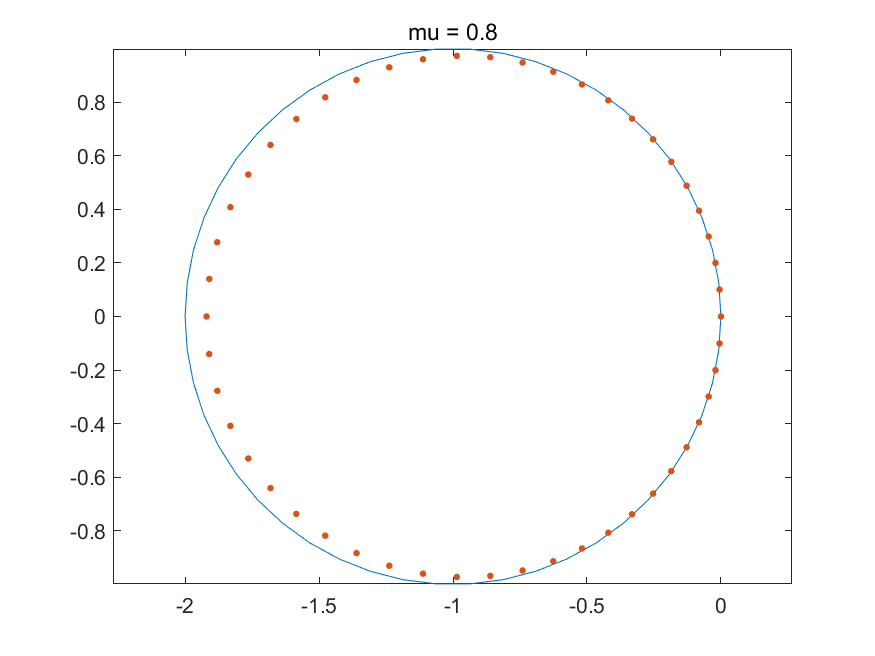
\includegraphics[width=\textwidth]{mu_0.8.png}
      \caption{$\mu=0.8$}
  \end{subfigure}
  \begin{subfigure}[b]{0.45\textwidth}
      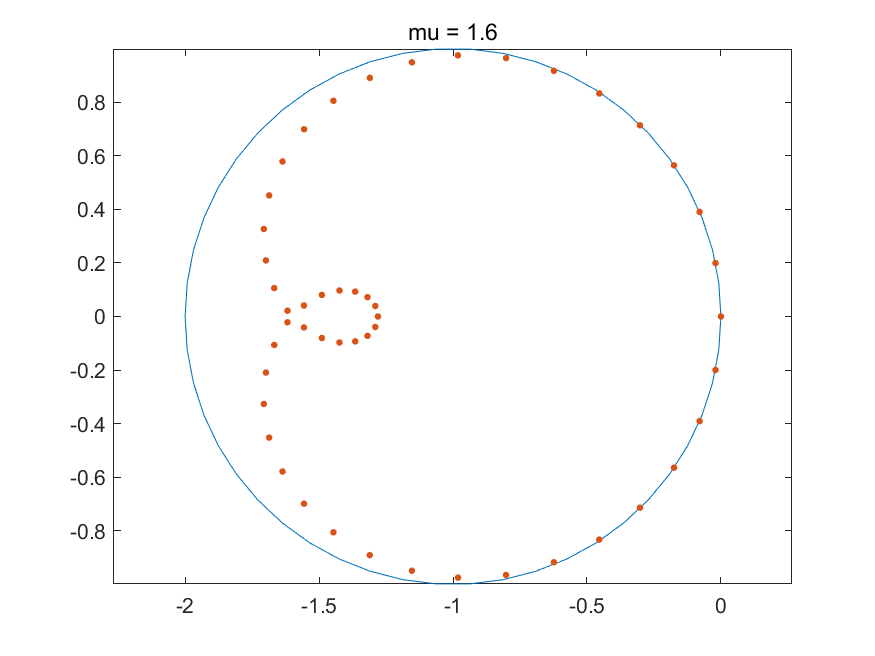
\includegraphics[width=\textwidth]{mu_1.6.png}
      \caption{$\mu=1.6$}
  \end{subfigure}
  \\
  \begin{subfigure}[b]{0.45\textwidth}
      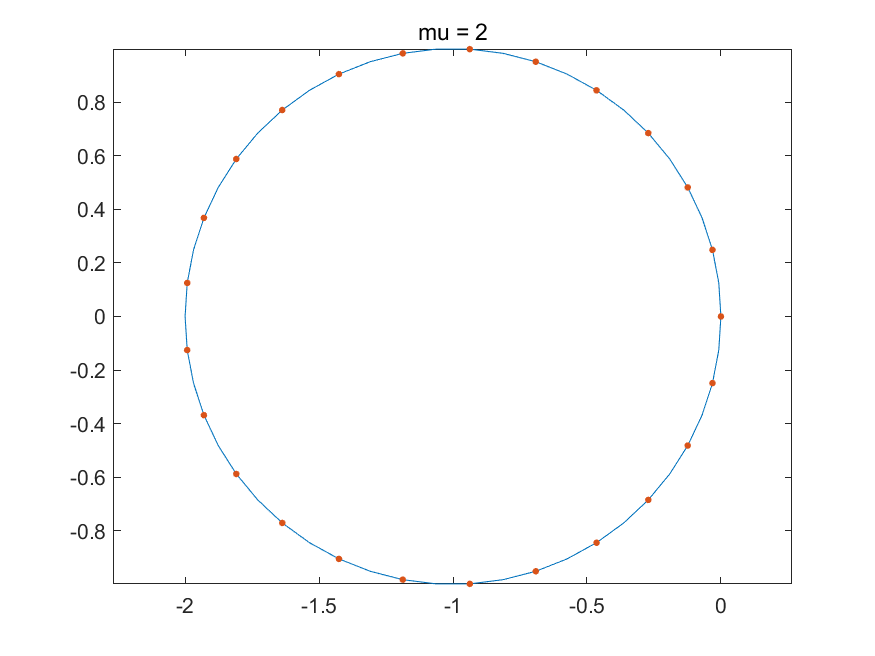
\includegraphics[width=\textwidth]{mu_2.png}
      \caption{$\mu=2$}
  \end{subfigure}
  \begin{subfigure}[b]{0.45\textwidth}
      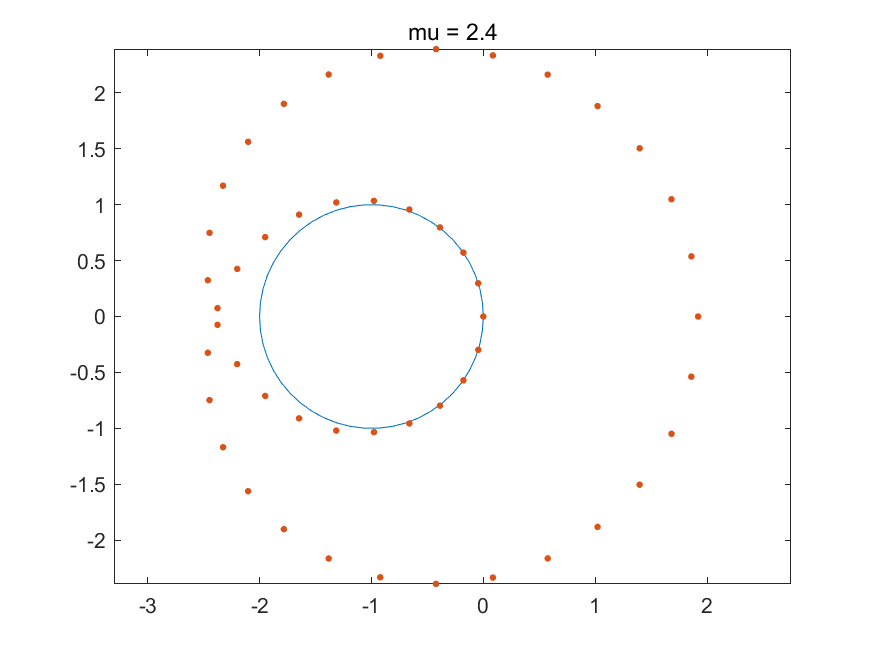
\includegraphics[width=\textwidth]{mu_2.4.png}
      \caption{$\mu=2.4$}
  \end{subfigure}
  \caption{Beam-Warming 方法的$z_p$示意图}
\end{figure}

\section{Exercise 12.87}
对于$\mu=0$,有决定域为
\begin{center}
  \begin{tikzpicture}
    \draw[step=1cm,dashed,gray,very thin] (0,0) grid (6,3);
    \fill (3, 0) circle (2pt);
    \fill (3, 1) circle (2pt);
    \fill (3, 2) circle (2pt);
    \fill (3, 3) circle (2pt);
    \coordinate [label=below:$x_j$] (A) at (3,0);
    \coordinate [label=left:$t_0$] (B) at (0,0);
    \coordinate [label=left:$t_3$] (C) at (0,3);
    \coordinate [label=right:$x_{j+3}$] (D) at (6,0);
  \end{tikzpicture}
\end{center}

对于$\mu=-1$,有决定域为
\begin{center}
  \begin{tikzpicture}
    \draw[step=1cm,dashed,gray,very thin] (0,0) grid (6,3);
    \fill (6, 0) circle (2pt);
    \fill (5, 1) circle (2pt);
    \fill (4, 2) circle (2pt);
    \fill (3, 3) circle (2pt);
    \coordinate [label=below:$x_j$] (A) at (3,0);
    \coordinate [label=left:$t_0$] (B) at (0,0);
    \coordinate [label=left:$t_3$] (C) at (0,3);
    \coordinate [label=right:$x_{j+3}$] (D) at (6,0);
  \end{tikzpicture}
\end{center}

对于$\mu=-2$,则有$U^{n+1}_j = 2U^{n}_{j+1} - U_j^n$,故决定域为
  \begin{center}
    \begin{tikzpicture}
      \draw[step=1cm,dashed,gray,very thin] (0,0) grid (6,3);
      \fill (3, 0) circle (2pt);
      \fill (4, 0) circle (2pt);
      \fill (5, 0) circle (2pt);
      \fill (6, 0) circle (2pt);
      \fill (3, 1) circle (2pt);
      \fill (4, 1) circle (2pt);
      \fill (5, 1) circle (2pt);
      \fill (3, 2) circle (2pt);
      \fill (4, 2) circle (2pt);
      \fill (3, 3) circle (2pt);
      \coordinate [label=below:$x_j$] (A) at (3,0);
      \coordinate [label=left:$t_0$] (B) at (0,0);
      \coordinate [label=left:$t_3$] (C) at (0,3);
      \coordinate [label=right:$x_{j+3}$] (D) at (6,0);
    \end{tikzpicture}
  \end{center}
  \section{Exercise 12.89}
  
  对于$\mu=1$,有$U^{n+1}_j = U^n_{j-1}$,故决定域为
  \begin{center}
      \begin{tikzpicture}
        \draw[step=1cm,dashed,gray,very thin] (0,0) grid (6,3);
        \fill (0, 0) circle (2pt);
        \fill (1, 1) circle (2pt);
        \fill (2, 2) circle (2pt);
        \fill (3, 3) circle (2pt);
        \coordinate [label=below:$x_j$] (A) at (3,0);
        \coordinate [label=left:$t_0$] (B) at (0,0);
        \coordinate [label=left:$t_3$] (C) at (0,3);
        \coordinate [label=right:$x_{j+3}$] (D) at (6,0);
      \end{tikzpicture}
    \end{center}

    对于$\mu=-1$,有$U^{n+1}_j = U^n_{j+1}$,故决定域为
\begin{center}
    \begin{tikzpicture}
      \draw[step=1cm,dashed,gray,very thin] (0,0) grid (6,3);
      \fill (6, 0) circle (2pt);
      \fill (5, 1) circle (2pt);
      \fill (4, 2) circle (2pt);
      \fill (3, 3) circle (2pt);
      \coordinate [label=below:$x_j$] (A) at (3,0);
      \coordinate [label=left:$t_0$] (B) at (0,0);
      \coordinate [label=left:$t_3$] (C) at (0,3);
      \coordinate [label=right:$x_{j+3}$] (D) at (6,0);
    \end{tikzpicture}
  \end{center}


  \section{Exercise 12.98}
  首先,我们展开Leapfrog方法的方程,用$v(x,t)$代替$U^n_j$,得到
$$
\frac{v(x, t+k) - v(x,t - k)}{2k} = -\frac{a}{2h}(v(x+h, t) - v(x-h, t))
$$

然后,将所有项在$(x,t)$处进行泰勒级数展开:

$$
\begin{aligned}
&\frac{1}{2}\left(\frac{v(x, t+k) - v(x, t)}{k} + \frac{v(x,t) - v(x,t - k)}{k}\right) \
&= v_t+\frac{1}{6}k^2v_{ttt}\
&= -a(v_x + \frac{h^2}{6}v_{xxx})+O(k^3)
\end{aligned}
$$

由$v_{ttt} = -a^3v_{xxx} + O(k^3)$,我们有

$$
v_t + av_x = \frac{k^2}{6}v_{ttt} -\frac{ah^2}{6}v_{xxx} + O(k^3) = \frac{ah^2}{6}(\mu^2 - 1)v_{xxx} + O(k^3)
$$

因此,Leapfrog方法的修正方程为(12.94)。


\section{Exercise 12.99}
由

$$
v_j^{n+1} = v_j^n - \frac{a\Delta t}{2\Delta x}(3v_j^n - 4v_{j-1}^n + v_{j-2}^n) + \frac{a^2\Delta t^2}{2\Delta x^2}(v_{j-2}^n - 2v_{j-1}^n + v_j^n)
$$

将$v_j^n$替换为$v(x,t)$,然后对该方程进行泰勒展开,得到:

$$
\begin{aligned}
v_t + av_x + \frac{ah^2}{6}(1-\mu)(1-2\mu)\frac{\partial^3 v}{\partial x^3} + O(\Delta t^2, \Delta x^3)
= v_t + av_x + \frac{ah^2}{6}(1-\mu)(1-2\mu)v_{xxx} + O(\Delta t^2, \Delta x^3)
\end{aligned}
$$

因此,Beam-Warming方法的修正方程为:

$$
v_t + av_x + \frac{ah^2}{6}(1-\mu)(1-2\mu)v_{xxx} = 0
$$

故 $a_1 = a, a_3 = - \frac{ah^2}{6}(\mu-1)(\mu-2)$, 由(F.46)
$$\omega(\xi) = a_1\xi + a_3\xi^3 = a\xi - \frac{ah^2}{6}(\mu-1)(\mu-2)\xi^3$$

代入得到$$\begin{aligned}
  &C_p(\xi) = \frac{\omega(\xi)}{\xi} = a + \frac{ah^2}{6}(\mu-1)(\mu-2)\xi^2\\
  &C_g(\xi) = \frac{d\omega}{d\xi} = a + \frac{ah^2}{2}(\mu-1)(\mu-2)\xi^2
\end{aligned}$$

\section{Exercise 12.100}
当$\mu = 1$时,Lax-Wendroff方法和Leapfrog方法的修正方程都变为了标准的对流方程$v_t + av_x = 0$,即它们成为了该方程的精确解。这意味着当$\mu = 1$时,两种方法都是精确的。

因为两种方法都是精确的,所以他们比$k=0.8h$时的效果好。
\section{Exercise 12.102}
$$
v_j^{n+1} = \frac{1}{2}(v_{j+1}^n + v_{j-1}^n) - \frac{\mu}{2}(v_{j+1}^n - v_{j-1}^n)
$$

其中$\mu = \frac{ak}{h}$。

为了应用von Neumann分析,我们假设$v_j^n = g(\xi)^ne^{i\xi jh}$,其中$\xi$是波数。将其代入Lax-Friedrichs方法中,我们得到:

$$
g(\xi)^{n+1}e^{i\xi jh} = \frac{1}{2}(g(\xi)^ne^{i\xi(j+1)h} + g(\xi)^ne^{i\xi(j-1)h}) - \frac{\mu}{2}(g(\xi)^ne^{i\xi(j+1)h} - g(\xi)^ne^{i\xi(j-1)h})
$$

简化这个表达式,我们得到:

$$
g(\xi) = \frac{1}{2}(1+\mu e^{-i\xi h}) \pm \frac{1}{2}\sqrt{(1-\mu e^{-i\xi h})^2 - 4\mu^2\sin^2(\xi h/2)}
$$

为了进一步简化这个表达式,我们可以使用恒等式$\cos\theta = \frac{1}{2}(e^{i\theta} + e^{-i\theta})$和$\sin\theta = \frac{1}{2i}(e^{i\theta} - e^{-i\theta})$。这给出了:

$$
g(\xi) = \cos(\xi h) - i\mu\sin(\xi h)
$$

这是式(12.99)中给出的放大因子。

为了找到稳定性条件,我们需要确保对于所有的$\xi$,$|g(\xi)| \leq 1$。这给出了:

$$
|g(\xi)|^2 = \cos^2(\xi h) + \mu^2\sin^2(\xi h) \leq 1
$$

简化这个不等式,我们得到:

$$
\mu^2 \leq 1 - \cos^2(\xi h) = \sin^2(\xi h)
$$

这个不等式对于所有的$\xi$成立,当且仅当$\mu \leq 1$。因此,Lax-Friedrichs方法仅在$\mu \leq 1$时稳定。
\section{Exercise 12.103}

$$
v_j^{n+1} = v_j^n - \frac{\mu}{2}(v_{j+1}^n - v_{j-1}^n) + \frac{\mu^2}{2}(v_{j+1}^n - 2v_j^n + v_{j-1}^n)
$$

其中,$\mu = \frac{ak}{h}$。

为了应用von Neumann分析,我们假设$v_j^n = g(\xi)^ne^{i\xi jh}$,其中$\xi$是波数。将其代入Lax-Wendroff方法中,我们得到:

$$
g(\xi)^{n+1}e^{i\xi jh} = g(\xi)^ne^{i\xi jh} - \frac{\mu}{2}(g(\xi)^ne^{i\xi(j+1)h} - g(\xi)^ne^{i\xi(j-1)h}) + \frac{\mu^2}{2}(g(\xi)^ne^{i\xi(j+1)h} - 2g(\xi)^ne^{i\xi jh} + g(\xi)^ne^{i\xi(j-1)h})
$$

简化这个表达式,我们得到:

$$
g(\xi) = 1 - i\mu\sin(\xi h) - 2\mu^2\sin^2(\xi h/2)
$$

这是式(12.100)中给出的放大因子。

为了找到稳定性条件,我们需要确保对于所有的$\xi$,$|g(\xi)| \leq 1$。这给出了:

$$
|g(\xi)|^2 = (1 - 2\mu^2\sin^2(\xi h/2))^2 + \mu^2\sin^2(\xi h) \leq 1
$$

简化这个不等式,我们得到:

$$
\mu^2 \leq \frac{1}{2}
$$

这个不等式对于所有的$\xi$成立,当且仅当$\mu^2 \leq \frac{1}{2}$。因此,Lax-Wendroff方法仅在$0 < \mu^2 \leq \frac{1}{2}$时稳定。
\end{document}